\documentclass[11pt,a4paper]{article}
\usepackage[T1]{fontenc}
\usepackage[utf8]{inputenc}
\usepackage{lmodern}
\usepackage[margin=2.5cm]{geometry}
\usepackage{amsmath,amssymb}
\usepackage{booktabs}
\usepackage{graphicx}
\usepackage[hidelinks]{hyperref}
\hypersetup{pdfauthor={Gianni Pilotti},pdftitle={Option Pricing in Python: Six Models Checked Against Each Other},pdfcreator={},pdfproducer={}}
\setlength{\parindent}{0pt}
\setlength{\parskip}{6pt}

\title{Option Pricing in Python:\\Six Models Checked Against Each Other}
\author{Gianni Pilotti}
\date{}

\begin{document}
\maketitle

\section{The Core Idea}
A pricing model is only useful if its output can be trusted. The repository builds six small pricers from scratch (Black-Scholes, binomial tree, Greeks, a barrier option, delta hedging, option strategies) and checks each one against a second method.

All notebooks use the same inputs: spot $S=100$, strike $K=100$, rate $r=3\%$ and volatility $\sigma=20\%$. Maturity is one year, except for the hedging and strategy notebooks (three months).

\begin{itemize}
\item \textbf{Closed form against numerics:} the tree converges to Black-Scholes, the Greeks match finite differences, the barrier formula matches Monte Carlo.
\item \textbf{Model against hedge:} a short call hedged with the model's own delta should end with a P\&L close to zero, and the error should shrink with more rebalancing.
\end{itemize}

\section{Method}
\subsection{Black-Scholes and implied volatility}
With $d_1=\dfrac{\ln(S/K)+(r+\tfrac12\sigma^2)T}{\sigma\sqrt T}$ and $d_2=d_1-\sigma\sqrt T$:
\[
C=S\,N(d_1)-Ke^{-rT}N(d_2),\qquad
P=Ke^{-rT}N(-d_2)-S\,N(-d_1).
\]
Put-call parity $C-P=S-Ke^{-rT}$ holds for any volatility and is used as a check. The implied volatility is the root of $C(\sigma)-C_{mkt}=0$ found with Brent's method on $[0.0001,\,5]$.

\subsection{Binomial tree (Cox-Ross-Rubinstein)}
With $n$ steps and $\Delta t=T/n$:
\[
u=e^{\sigma\sqrt{\Delta t}},\quad d=1/u,\quad p=\frac{e^{r\Delta t}-d}{u-d},\quad
V_t=e^{-r\Delta t}\left(pV_{t+1}^{up}+(1-p)V_{t+1}^{down}\right).
\]
For an American option, the value at each node is $\max(V_t,\ \text{intrinsic value})$.

\subsection{Greeks}
Closed forms for the call, with $\varphi$ the normal density, in the units used by the code:
\begin{gather*}
\Delta=N(d_1),\qquad
\Gamma=\frac{\varphi(d_1)}{S\sigma\sqrt T},\qquad
\mathcal{V}=\frac{S\varphi(d_1)\sqrt T}{100},\\
\Theta=\frac{1}{365}\left(-\frac{S\varphi(d_1)\sigma}{2\sqrt T}-rKe^{-rT}N(d_2)\right),\qquad
\rho=\frac{KTe^{-rT}N(d_2)}{100}.
\end{gather*}
Vega is per vol point, theta per calendar day and rho per 1\% of rate. Each is compared with a central finite difference with a bump of $10^{-4}$.

\subsection{Down-and-out call}
For a barrier $H\le K$ watched continuously, the price is the vanilla call minus the down-and-in call. With $\lambda=(r+\tfrac12\sigma^2)/\sigma^2$ and $y=\dfrac{\ln(H^2/(SK))}{\sigma\sqrt T}+\lambda\sigma\sqrt T$:
\[
C_{DI}=S\left(\tfrac HS\right)^{2\lambda}N(y)-Ke^{-rT}\left(\tfrac HS\right)^{2\lambda-2}N(y-\sigma\sqrt T),\qquad
C_{DO}=C-C_{DI}.
\]
The Monte Carlo uses 100,000 paths of 252 daily steps (seed 1) and sets the payoff to zero if any daily price is at or below $H$. Daily monitoring is less strict than continuous monitoring, so the simulated price is higher. The Broadie-Glasserman-Kou correction moves the barrier to $H\,e^{-0.5826\,\sigma\sqrt{\Delta t}}$ in the formula.

\subsection{Delta hedging and strategies}
The seller of a call receives the premium, buys $\Delta$ shares and rebalances at $n$ equal dates. Cash grows at $r$. At expiry the final P\&L is
\[
\text{P\&L}=\text{cash}_T+\Delta_{n-1}S_T-\max(S_T-K,0).
\]
There are no costs or dividends. The test uses a 3-month at-the-money call, 2,000 simulated paths per case and seed 7.

For strategies, each leg is a (type, strike, quantity). The profit at expiry is $\sum_i q_i\,\text{payoff}_i(S_T)-\text{cost}\times e^{rT}$, where the cost is the sum of Black-Scholes prices. Break-evens are the sign changes on a grid of 1,601 prices between 60 and 140.

\section{Results}
\textbf{Tree against Black-Scholes} (ATM call, 1 year, Black-Scholes price 9.4134):

\begin{center}
\begin{tabular}{@{}rcc@{}}
\toprule
Steps & Tree price & Error \\
\midrule
10 & 9.2179 & $-0.1956$ \\
100 & 9.3936 & $-0.0198$ \\
1000 & 9.4114 & $-0.0020$ \\
\bottomrule
\end{tabular}
\end{center}
The error falls roughly in proportion to $1/n$ (ten times more steps, ten times smaller error).

\textbf{American against European puts} (500 steps). An American call without dividends has the same value as the European call (9.4094 for both).

\begin{center}
\begin{tabular}{@{}rccc@{}}
\toprule
Strike & European put & American put & Early exercise premium \\
\midrule
80 & 0.8607 & 0.8830 & 0.0223 \\
100 & 6.4540 & 6.7411 & 0.2871 \\
120 & 19.2195 & 20.6068 & 1.3873 \\
140 & 36.4932 & 40.0000 & 3.5068 \\
\bottomrule
\end{tabular}
\end{center}
At $K=140$ the American put is worth its intrinsic value of 40: it is optimal to exercise at once.

\textbf{Greeks.} The formula and the finite difference agree to five decimals for the ATM call: delta 0.59871, gamma 0.01933, vega 0.38667, theta $-0.01474$ and rho 0.50457.

\textbf{Barrier} ($H=90$): the vanilla call is 9.4134. The down-and-out call is 7.7402 by formula. Monte Carlo gives 8.0034 (95\% interval $\pm0.0869$). The formula with the adjusted barrier gives 7.9700, which is inside the Monte Carlo interval.

\textbf{Delta hedging} (call sold for 4.3576):

\begin{center}
\begin{tabular}{@{}rcc@{}}
\toprule
Rebalances & Mean P\&L & Std P\&L \\
\midrule
4 & $+0.0445$ & 1.5724 \\
13 & $+0.0112$ & 0.9449 \\
63 & $-0.0004$ & 0.4349 \\
252 & $+0.0023$ & 0.2199 \\
\bottomrule
\end{tabular}
\end{center}

\begin{figure}[h]
\centering
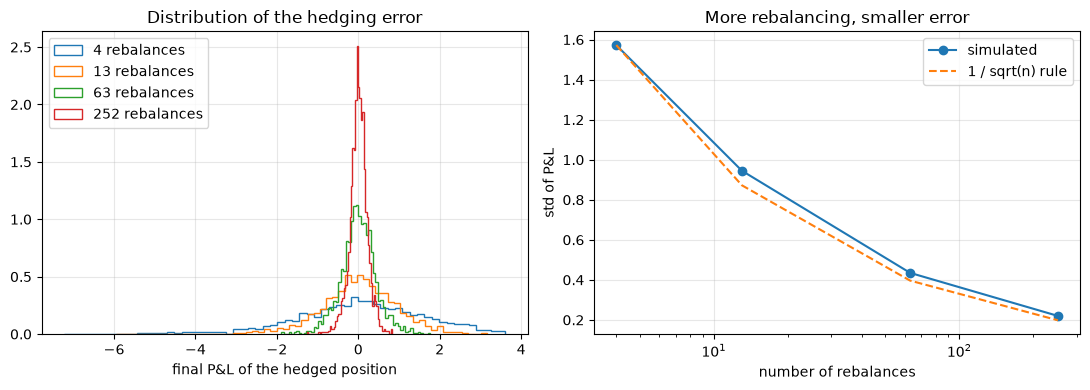
\includegraphics[width=0.95\textwidth]{../figures/05_1.png}
\caption{Distribution of the hedging error (left) and its standard deviation against the $1/\sqrt n$ rule (right).}
\end{figure}

\textbf{Strategies} (3 months, strikes in brackets; a negative cost is a credit):

\begin{center}
\begin{tabular}{@{}lrrrl@{}}
\toprule
Strategy & Cost & Max profit & Max loss & Break-even \\
\midrule
Bull call spread (95/105) & 5.07 & 4.89 & $-5.11$ & 100.1 \\
Long straddle (100) & 7.97 & unlimited & $-8.03$ & 92.0, 108.0 \\
Long strangle (95/105) & 3.98 & unlimited & $-4.01$ & 91.0, 109.0 \\
Butterfly (90/100/110) & 3.66 & 6.31 & $-3.69$ & 93.7, 106.3 \\
Iron condor (85/90/110/115) & $-1.07$ & 1.08 & $-3.92$ & 88.9, 111.1 \\
\bottomrule
\end{tabular}
\end{center}

\section{Worked Example}
\textbf{Black-Scholes by hand} for $S=K=100$, $T=1$, $r=3\%$, $\sigma=20\%$:
\begin{align*}
d_1&=\frac{0+(0.03+0.02)\times1}{0.20}=0.25,\qquad d_2=0.25-0.20=0.05,\\
N(d_1)&=0.59871,\qquad N(d_2)=0.51994,\qquad Ke^{-rT}=97.0446,\\
C&=100\times0.59871-97.0446\times0.51994=59.871-50.457=9.4134.
\end{align*}
The put is $97.0446\times0.48006-100\times0.40129=6.4580$. Parity: $9.4134-6.4580=2.9554=100-97.0446$. The numbers $N(d_1)=0.59871$ and $N(d_2)=0.51994$ also give the delta and, through $KTe^{-rT}N(d_2)/100$, the rho of 0.50457 in the Greeks results above.

\textbf{Barrier correction.} For daily monitoring, $\sigma\sqrt{\Delta t}=0.20\times\sqrt{1/252}=0.01260$, so
\[
H_{adj}=90\times e^{-0.5826\times0.01260}=90\times e^{-0.00734}=89.34 .
\]
Lowering the barrier makes the option less likely to be knocked out, so the price rises from 7.7402 to 7.9700.

\textbf{The $1/\sqrt n$ rule.} From 4 rebalances (std 1.5724), the rule predicts $1.5724\times\sqrt{4/252}=0.198$ at 252 rebalances. The simulation gives 0.2199, about 11\% higher.

\section{Limits}
\begin{itemize}
\item \textbf{Textbook assumptions:} constant volatility and rate, no dividends, no transaction costs, and continuous trading in the limit. Real markets have a smile and costs.
\item \textbf{Small samples:} the hedging test uses 2,000 paths per case and one seed. The mean P\&L values of 0.0445 against 0.0023 are noise of the order of the standard error (about 0.035 for 4 rebalances).
\item \textbf{Barrier monitoring:} the Monte Carlo with 252 steps sits 0.033 above the corrected formula. The correction is an approximation.
\item \textbf{No market data:} all prices are model prices, so the notebooks check internal consistency, not agreement with traded prices. These are model outputs, not recommendations.
\end{itemize}

\end{document}
